\documentclass[a4paper, 12pt]{article}
\usepackage[utf8]{inputenc}
\usepackage[top=2cm, botttom=2cm, left=2.5cm, right=2.5cm]{geometry}
\usepackage{float}
\usepackage{graphicx}
\usepackage[brazil]{babel}
\begin{document}

\title{PI Final}
\author{Victor Yassunori Okada\\Ciência da Computação 1º Semestre\\CENTRO UNIVERSITÁRIO SENAC}
\date{São Paulo, 14 de Junho 2020}
 \begin{figure}
        \centering
        
\includegraphics[scale=0.1]{Senac-logo.jpg}
        \label{fig:my_label}
    \end{figure}


\maketitle
 \newpage
 \tableofcontents \newpage



 \newpage
\section{INTRODUÇÃO}

Os carros automatizados - também conhecidos como veículos robóticos (tema central apresentado inicialmente ao mundo em 1939 na Feira Mundial de Nova Iorque pela empresa Futurama) - deram início à um tema - o qual vem sendo não só analisado e discutido, como também pesquisado por grandes empresas multinacionais de tecnologia ao longo dos anos seguintes -  desenvolvendo protótipos como ocorreu pela empresa Tesla em meados de 2016. 
A empresa Tesla se destacou em lançar o mais novo modelo de sua linha: O Tesla S, que promete fazer até 600km por carga, silencia ruídos do carro durante o passeio e ao mesmo tempo promete aumento de velocidade. No entanto, houve grande repercussão após a morte de Joshua Brown, um americano de 40 anos, que morreu a bordo do mesmo, no piloto automático em um acidente envolvendo um caminhão - o qual passou despercebido pelos mecanismos de tecnologia de sensores do veículo - ocasionando o desastre que colocaria a incerteza da viabilidade dos carros autônomos com relação à imprevisibilidade das ações humanas no cotidiano. 
Desta maneira, muitos temas acabam por se tornarem evidentes em relação aos novos meios de transporte automatizados, que por sua vez podem trazer muitos benefícios ao meio ambiente e mobilidade humana dentre diversos outros aspectos, como também incontáveis desvantagens aos mesmos.
Neste sentido, o presente trabalho tem como finalidade apresentar o tema “Carros Autônomos” objetivando seu desenvolvimento e ação em correlação à vida no globo, onde encontram-se diversas formas de vidas e suas respectivas necessidades em mutualismo ao meio ambiente.
 \newpage
 
\section{ORIGEM E HISTÓRIA}


    Desde a Antiguidade o homem já se locomovia através de trenós primitivos puxados por animais robustos (bisões, bois, etc.). Porém, sua velocidade de locomoção era muito baixa se compararmos com a invenção da roda em 3500 a.C -  considerada pela maioria dos historiadores “a maior invenção do homem até então” – pois permitiu o mesmo a se locomover e se desenvolver em diversas regiões do planeta.
    A partir disso, temos a criação de veículos primitivos - principalmente aqueles usados em guerras famosas como Roma, Grécia Antiga e Reconquista - e sua consequente evolução a partir de meados do século XVIII, onde tivemos por subsequente a maior revolução socioeconômica da história humana: A Revolução Industrial de 1750.
    A Revolução Industrial, permitiu ao homem - em meados dos séculos XVIII-XIX – o desenvolvimento de máquinas a vapor e veículos automotivos movidos a combustíveis fósseis (carvão mineral, petróleo). Segundo o historiador brasileiro Gilberto Cotrim: “a Revolução Industrial propiciou o homem a recomeçar sua história de produção do zero”.
    Com o surgimento do Fordismo no início do século XX, temos como destaque a introdução de uma linha de produção semi-automatizada e focada em uma produção em massa para atendimento de uma demanda capitalista crescente. Mais tarde, temos a aplicação do Taylorismo nas fábricas Ford em busca de melhores administrações para a empresa, que permitiu a racionalização do trabalho nas fábricas, criando assim a divisão do trabalho.
    
    \begin{figure}[htb]
        \centering
        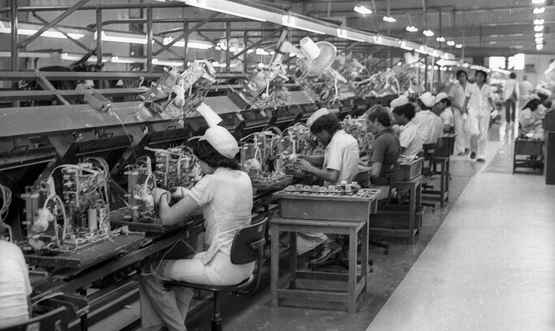
\includegraphics[scale=0.5]{0001.png}
        \caption{Produção em larga-escala à partir da Revolução Industrial}
        \label{fig:my_label}
    \end{figure}
    
    O século XX foi marcado pelo embasamento de guerras mundiais e semi-guerras, a maioria delas disputando meios de artilharia superiores para ser objetivados nos campos de batalha. Temos nos anos 70 a conhecida guerra do Golfo, que freou por definitivo o fornecimento de combustíveis para o mundo. No Brasil, tivemos o surgimento do movimento Proálcool que tornou o nosso país independente para produção de combustíveis nacionais e a não-dependência de combustíveis estrangeiros.
    
    A transição dos séculos XX-XXI demarcou a importância da manutenção da camada de ozônio em meados dos anos 90, com a ECO-92, que promoveu a discussão em larga escala dos países do G7 da ONU (Estados Unidos, França, Alemanha, Japão, Reino Unido, Itália e Canadá), a entrarem em um acordo comum em relação as drásticas mudanças climáticas e a assinatura dos países em questão do Protocolo de Kyoto – que pretendia limitar a emissão de CO2 para cada país. Porém a venda dos famosos “créditos de carbono” de países de Terceiro Mundo para os países de Primeiro Mundo como os EUA, colocaram fim ao tratado.   
    Atualmente, vivenciamos a preocupação de renovação e preservação dos recursos naturais, devido à grande demanda de pessoas para um planeta limitado. Hoje, se tem como destaque, uma guerra entre países de Primeiro Mundo (EUA por exemplo), que recentemente com suas reservas hidrográficas escassas e com sua saída em 2018 do Acordo de Paris – acordo que propiciava a limitação de lançamento de poluentes na atmosfera por parte dos países de Primeiro Mundo (semelhante ao protocolo de Kyoto de 1992) -  teve-se por sua vez a iniciativa do presidente americano Donald Trump, de se explorar as reservas de gás xisto – que são atualmente um dos maiores poluentes do planeta (sendo equivalente a 3 vezes mais poluente do que o Co2) -  para suprir  as demandas energéticas do país.

    O lançamento de carros elétricos revolucionou o mercado devido a ascensão da escassez de combustíveis fosseis no mundo e a procura da restauração socioambiental do mesmo. A empresa Google lançou, em meados de 2010, o primeiro veículo autônomo, onde se têm um monitoramento inteligente, com radares e câmeras controladas por profissionais de segurança por satélite. Seu destaque é sua visão inteligente (360 graus) que permite a identificação de buracos, acidentes, pedestres e semáforos, todo o tipo de irregularidades que preocupa um motorista comum.

      \begin{figure}[htb]
        \centering
        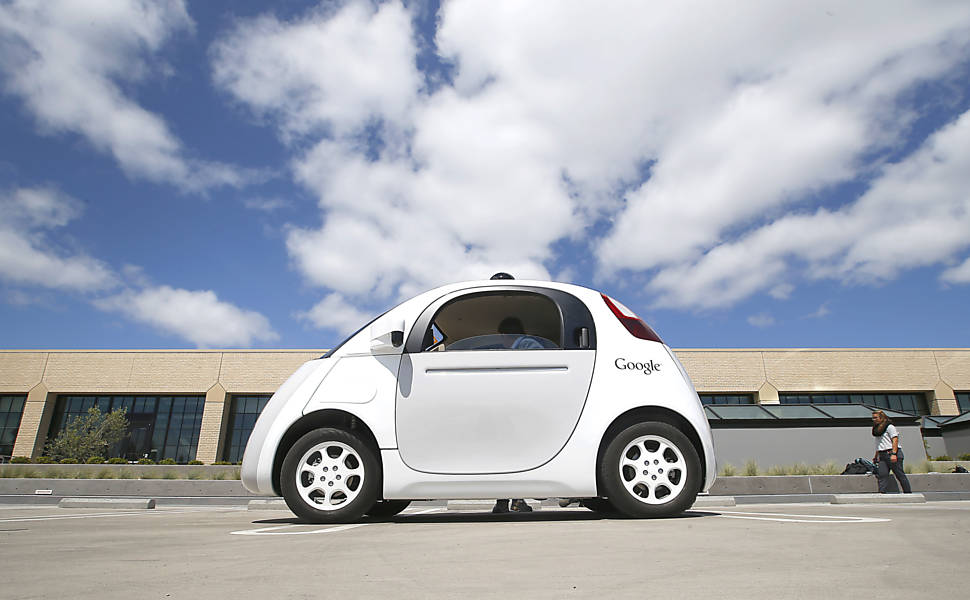
\includegraphics[scale=0.5]{0002.png}
        \caption{Carro automatizado lançado pela Google em 2009}
        \label{fig:my_label}
    \end{figure}
    
    Um exemplo de sistema autônomo inteligente é a mais nova linha 4 Amarela do metrô de São Paulo, que recebeu recentemente o certificado TUV, por ter o padrão de qualidade e segurança que um metrô autônomo precisa ter: passagem livre entre os carros; comunicação direta com o Centro de Controle Operacional (CCO); câmeras de segurança em cada carro monitoradas pelo CCO; baixo nível de ruído; ar condicionado; acessibilidade plena; portas frontais de emergência; sistema de iluminação com eficiência energética.
 \newpage
\section{FUNCIONABILIDADE}

    Como funcionam? Computadores diferenciam os tipos de obstáculos e de situações nas vias. Os computadores de bordo trocam informações entre si. Assim, um imprevisto ocorrido com um dos automóveis servirá para que todos aprendam a lidar com circunstâncias equivalentes. 
    
        \begin{figure}[htb]
        \centering
        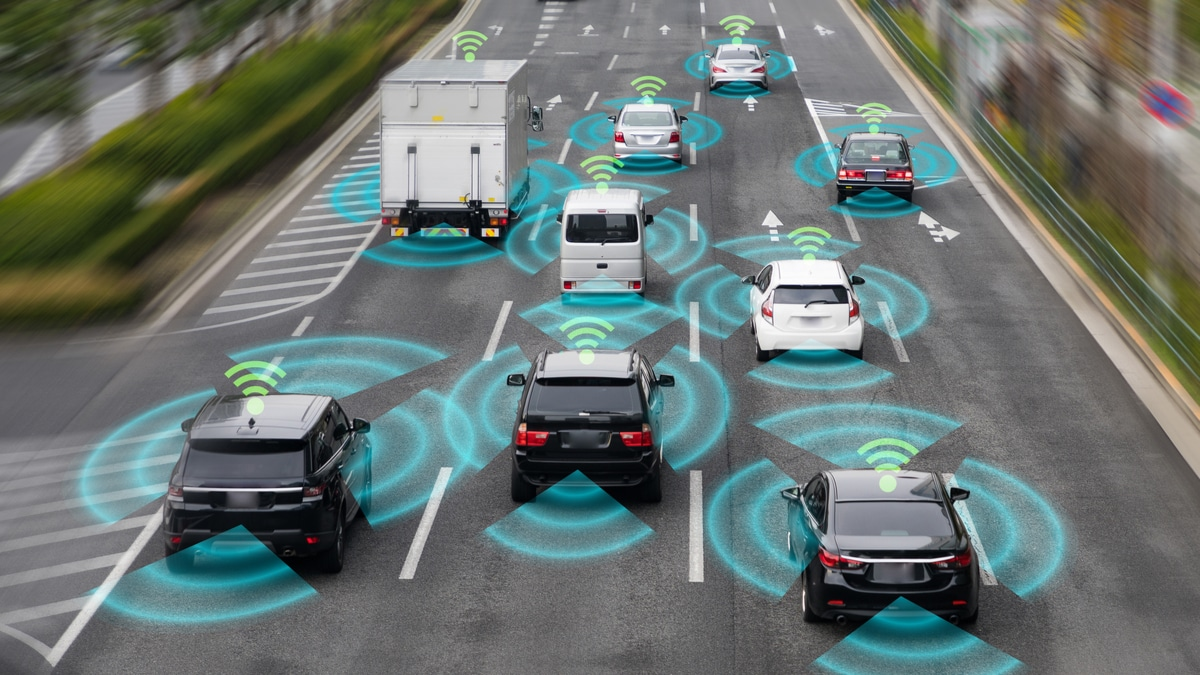
\includegraphics[scale=0.5]{0003.png}
        \caption{Exemplo de sensores de carros automatizados}
        \label{fig:my_label}
    \end{figure}
    
    Diversos componentes trabalham em conjunto para garantir que um carro autônomo tenha a percepção e a orientação necessárias a uma direção segura. Câmeras, sensores e radares funcionam como os olhos do veículo, detectando obstáculos, sinais de trânsito, semáforos, pedestres, relevo etc.

    A grande vantagem é que esses equipamentos fazem uma verdadeira varredura ao redor do veículo, permitindo que ele enxergue em 360 graus. Desse modo, ele pode perceber situações que dificilmente o olho humano conseguiria captar, aumentando consideravelmente a segurança dos carros autônomos.
    
    O que muda com a chegada dos carros autônomos no mercado? popularização dos carros autônomos tem a capacidade de revolucionar o mercado automotivo. Isso porque boa parte das interações entre humanos e veículos será substituída pela autonomia de seus sistemas. 

    Assim, com menos erros humanos e maior conhecimento e experiência acumulados, desgastes, quebras e falhas tendem a ser menos recorrentes, impactando todo o setor automotivo.
     \newpage
    \section{A VIABILIDADE DOS VEÍCULOS AUTÔNOMOS}
    
     O desenvolvimento de novas tecnologias que por sua vez visam a inovação dentro da indústria/comércio automotivo cresce com o passar dos anos desde a origem do primeiro motor a vapor de automóveis em 1769, que possibilitou o início da mobilidade urbana no mundo.
     
    \begin{figure}[htb]
        \centering
        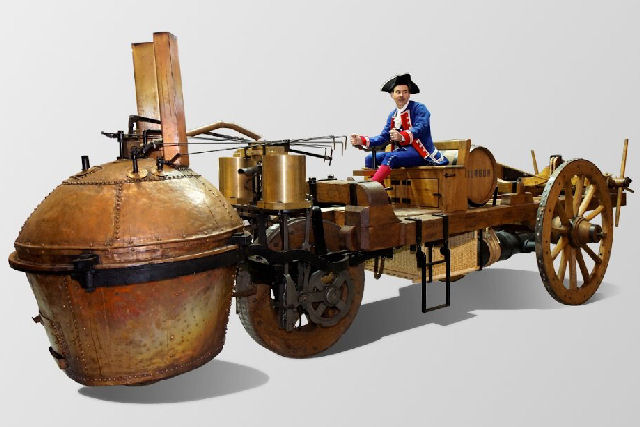
\includegraphics[scale=0.5]{0004.png}
        \label{fig:my_label}
    \end{figure}
    
    Com a expansão da inteligência artificial, a ideia de veículos automatizados que antes utópica, torna-se agora menos distante da realidade. Grandes Multinacionais da tecnologia automotiva, estão ativamente no desenvolvimento de veículos, os quais são desprovidos da carência de um motorista, podendo circular pelas estradas por meio de sensores e tecnologia de conectividade que dão ao veículo a possibilidade de percepção e interação com o meio ao seu redor. No entanto, uma controvérsia cabe aos cientistas computacionais por trás desta grande engenhosidade: a imprevisibilidade das ações e expressões do Reino Animal, grupo que compreende os seres vivos amparados da necessidade de locomoção para sua sobrevivência. É evidente que a presente tecnologia, independentemente de seu avanço, ainda não foi capaz de tornar suas decisões por si só, fato ilustrado na sua incapacidade de sortear elementos, realizando este ofício por meio de operações matemáticas pré-programadas.

    Considerando o exposto, é inevitável questionar sua viabilidade no atual contexto em que se encontra os limites que a tecnologia pode alcançar. Exemplificado no episódio ocorrido com o veículo Tesla Model S, mencionado anteriormente, o qual reprovou no quesito “segurança” defendido pela grande empresa de tecnologia automotiva Tesla.

    \begin{figure}[htb]
        \centering
        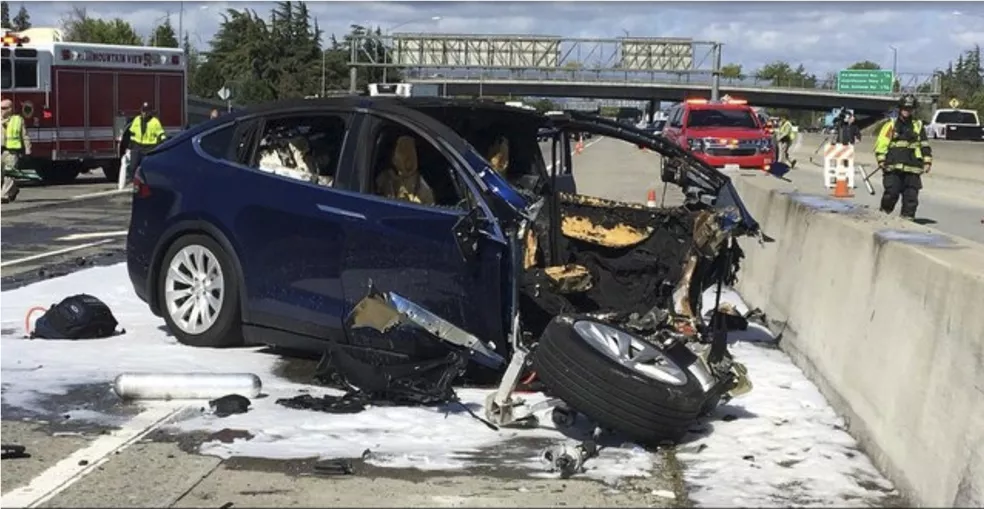
\includegraphics[scale=0.5]{0005.png}
        \caption{Acidente de carro provocado por falha de veículo automatizado pela fabricante Tesla}
        \label{fig:my_label}
    \end{figure}
    
    
    No entanto, é possível inferir suas vantagens com relação ao meio ambiente, uma vez que com os mesmos transitando, seria inviável a necessidade de automóveis particulares, sendo possível utilizar os seus serviços de locomoção por meio de aplicativos, cujos possibilitariam o encontro do automóvel ao usuário e consequentemente sua chegada ao destino desejável, reduzindo a frota e transito de carros existentes na malha de estradas e rodovias dos polos urbanos, diminuindo assim a liberação de gases poluentes na atmosfera.

    Portanto, é necessário não só um desenvolvimento da tecnologia de inteligência artificial nos carros automatizados como também um preparo dos meios urbanos para o concedimento destes veículos, para que ambos possam compartilhar informações mutuamente, por meio de sensores que captam informações e armazenem em seguida os dados coletados em servidores online, que por fim disponibilizam suas informações aos automóveis habilitados por meio da tecnologia das coisas, evitando futuros acidentes.
 \newpage
\section{CARROS AUTÔNOMOS NO BRASIL}

    Uma pesquisa realizada pela KPMG, em 2019, chamada “Autonomous vehicles readiness index”, investiga o preparo para introdução de veículos autônomos em diferentes países. Este estudo leva em conta quatro pilares: legislações governamentais, tecnologia e inovação, infraestrutura e aceitação do consumidor. Os dados colhidos apontam o Brasil como o país menos preparado, dentro dos 25 países selecionados, para receber os veículos autônomos.

    Essa tecnologia vem sendo desenvolvida em universidades brasileiras. Na Universidade Federal do Espírito Santo (UFES), foi criado um robô autônomo inteligente e no campus de São Carlos da universidade de São Paulo (UFScar), realizou-se um carro robótico para navegação autônoma. Isso indica que o país tem o potencial para desenvolver este tipo de tecnologia. No entanto, atualmente nos deparamos com um baixo incentivo do governo para o desenvolvimento do conhecimento científico, evidente nos cortes de bolsas para pesquisa. O estudo também aponta a baixa eficácia das políticas governamentais brasileiras de incentivo aos veículos autônomos bem como o investimento em infraestrutura para que isto se torne viável em um futuro próximo.

    Com relação ao interesse dos consumidores, Maurício Endo (sócio-líder de Governo e infraestrutura da KPMG no Brasil e na América Latina), aponta uma boa aceitação dos brasileiros para novas tecnologias. Portanto, se os veículos autônomos forem vendidos a um preço acessível, ele considera que a população rapidamente irá aderir a essa nova tecnologia. Em conclusão, podemos considerar que os principais impasses para a incorporação de veículos autônomos no Brasil correspondem ao baixo incentivo do governo para o tal.  
     \newpage
    \section{CONCLUSÃO}
    
    Reiteramos que o conveniente tema discutido nesse trabalho apresenta uma ambiguidade sugestiva e abarca uma série de discussões a ser tratada, devido a sua abrangência como fator socioeconômico e político – por se tratar de uma questão que envolve os mais diversos setores socioeconômicos de nossa sociedade e que necessita de uma conciliação entre os mesmos; assim como abrange uma questão política, pois exacerba uma questão de aceitação e conciliação desta em territórios federalizados ou como também ditatoriais – como demonstrado o caso Sophia – como também religioso – pois os religiosos detém, principalmente no Brasil, grande poder de veto em questões que envolvam o modo de vida de um cidadão como também sua atuação enquanto cidadãos.
    
    Indubitavelmente é necessária a manutenção de nossa sociedade de tempos em tempos, para que não fiquemos estagnados em uma forma de vida padronizada. Porém, é de grande importância nos desgarrarmos de nosso sentimento primitivo, onde Platão comenta em sua tese da Alegoria da Caverna: “O homem que permanece dentro da caverna é arrogante pois não conhece a luz da razão que há fora dela”.
     \newpage
    \section{BIBLIOGRAFIA:}
    
    https://home.kpmg/content/dam/kpmg/xx/pdf/2019/02/2019-autonomous-vehicles-readiness-index.pdf
    https://canaltech.com.br/carros/tesla-model-s-e-x-ganham-mais-autonomia-e-potencia-137823/
    https://jornal.usp.br/universidade/carro-autonomo-da-usp-ganha-premio-em-desafio-mundial/
    https://olhardigital.com.br/carros-e-tecnologia/noticia/intel-e-lideres-automotivos-definem-regras-para-carros-autonomos/87555
    https://www.vox.com/future-perfect/2020/2/14/21063487/self-driving-cars-autonomous-vehicles-waymo-cruise-uber
    https://revistacarro.com.br/
    https://waymo.com/tech/



\end{document}